\section{Test Procedures} % (fold)
\label{sec:test_procedures}

The following test procedures will be used to verify that each part of this laboratory exercise satisfies the requirements given in \hyperref[sec:requirements]{Section \ref*{sec:requirements}}.
Modules are to be tested beginning with lower-level modules and moving up so as to isolate issues in a module dependencies.

\subsection{PC Incrementer} % (fold)
\label{sub:pc_incrementer_procedure}

The following test procedure will be used to verify that the Verilog module, \verb|PCAdder|, satisfies the requirements for this part.

\begin{enumerate}
    \item The PC incrementer circuit will be tested using \emph{ModelSim} and the testbench shown in \hyperref[lst:testPCAdder]{Listing \ref*{lst:testPCAdder}}.
    This testbench generates the test vectors shown in \hyperref[tab:pcadder_vectors]{Table \ref*{tab:pcadder_vectors}} and outputs the output $O$.
    Simulations will be run in order to verify the behavior shown in \hyperref[tab:pcadder_vectors]{Table \ref*{tab:pcadder_vectors}}.
    \item Generate the test vectors shown in \hyperref[tab:pcadder_vectors]{Table \ref*{tab:pcadder_vectors}} and verify the corresponding outputs, $O$.
\end{enumerate}

\begin{table}[htbp]
    \centering
        \begin{tabular}{ll} \toprule
            $I$     & $O$   \\\midrule
            00000   & 00001 \\
            00001   & 00010 \\
            00010   & 00011 \\
            00011   & 00100 \\
            00100   & 00101 \\
            00101   & 00110 \\
            00110   & 00111 \\
            00111   & 01000 \\
            01000   & 01001 \\
            01001   & 01010 \\
            01010   & 01011 \\
            01011   & 01100 \\
            01100   & 01101 \\
            01101   & 01110 \\
            01110   & 01111 \\
            01111   & 10000 \\
            10000   & 10001 \\
            10001   & 10010 \\
            10010   & 10011 \\
            10011   & 10100 \\
            10100   & 10101 \\
            10101   & 10110 \\
            10110   & 10111 \\
            10111   & 11000 \\
            11000   & 11001 \\
            11001   & 11010 \\
            11010   & 11011 \\
            11011   & 11100 \\
            11100   & 11101 \\
            11101   & 11110 \\
            11110   & 11111 \\
            11111   & 00000 \\\bottomrule
        \end{tabular}
    \caption{PC Incrementer Test Vectors\label{tab:pcadder_vectors}}
\end{table}
% subsection pc_incrementer (end)

\subsection{Multiplexer} % (fold)
\label{sub:multiplexer}

The multiplexer module, \verb|PCUp|, was implemented from the \emph{Altera} library of parameterized modules (LPM).
It will therefore not be specifically tested.

% subsection multimplexer (end)

\subsection{Decoder} % (fold)
\label{sub:decoder}

The decoder module, \verb|DecoderN|, has been previously used and tested for Homework 6.
It will therefore not be specifically tested.
% subsection decoder (end)

\subsection{Register} % (fold)
\label{sub:register}

The register module, \verb|RegisterOEN|, has been previously used and tested for Homework 6 and only minimally modified.
It will therefore not be specifically tested.
% subsection register (end)

\FloatBarrier \subsection{Controller} % (fold)
\label{sub:controller_pro}

The following test procedure will be used to verify that the Verilog module, \verb|controller|, satisfies the requirements for this part.

\begin{enumerate}
    \item Ensure that the RTL view shows a state machine similar to that shown in \hyperref[fig:state_diagram]{Figure \ref*{fig:state_diagram}}.
\end{enumerate}

\begin{figure}[htbp]
    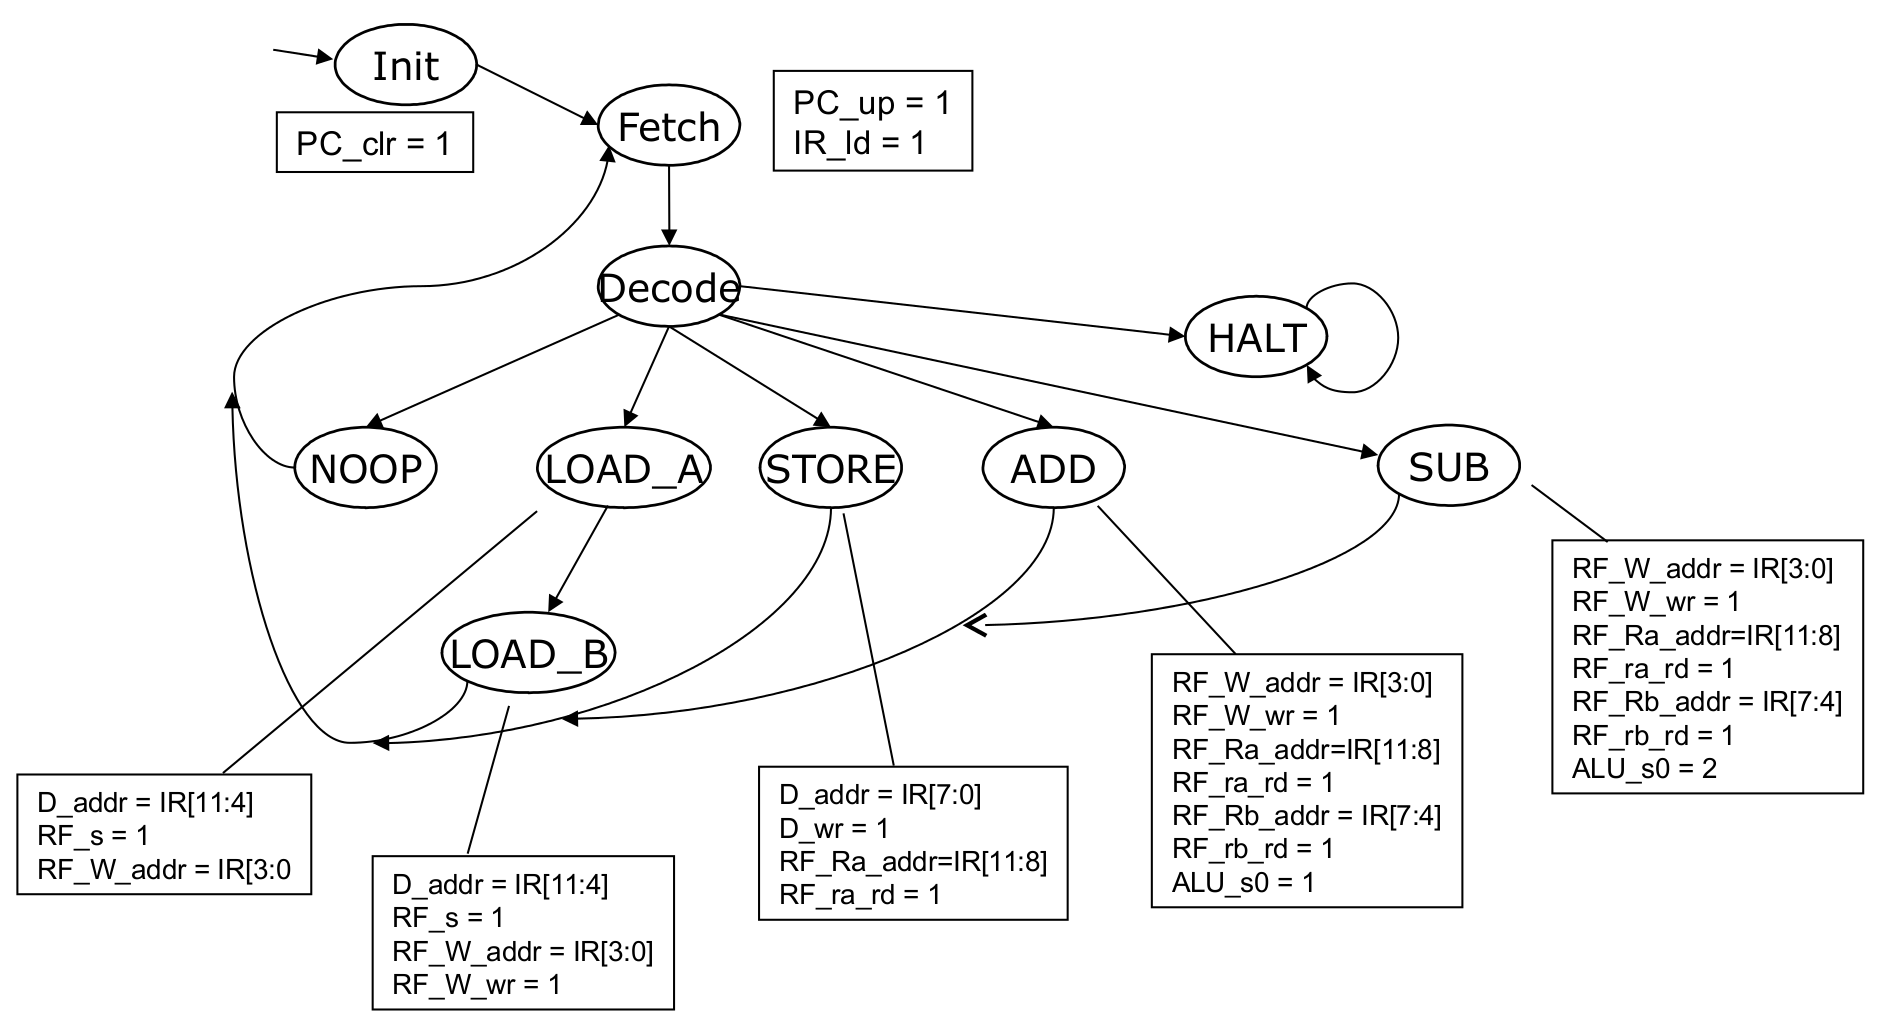
\includegraphics[width=\textwidth]{images/state_diagram.png}
    \caption{Controller State Diagram\label{fig:state_diagram}}
\end{figure}

% subsection controller (end)

\subsection{Program Counter} % (fold)
\label{sub:program_counter_pro}

The following test procedure will be used to verify that the Verilog module, \verb|PC|, satisfies the requirements for this part.

\begin{enumerate}
    \item The program counter circuit will be tested using \emph{ModelSim} and the testbench shown in \hyperref[lst:testPC]{Listing \ref*{lst:testPC}}.
    \item Generate sequantial values when the count enable signal is high and reset to zero on a high reset signal.
\end{enumerate}

% subsection program_counter (end)

\subsection{Instruction Memory} % (fold)
\label{sub:instruction_memory}

The instruction memory module, \verb|imemlpm| is implemented from the LPM.
It will therefore not be specifically tested.
% subsection instruction_memory (end)


\subsection{Instruction Register} % (fold)
\label{sub:instruction_register_pro}

The following test procedure will be used to verify that the Verilog module, \verb|instruction_register|, satisfies the requirements for this part.

\begin{enumerate}
    \item The instruction register circuit will be tested using \emph{ModelSim} and the testbench shown in \hyperref[lst:testir]{Listing \ref*{lst:testir}}.
    \item Ensure that a load is only succesful when the load enable signal is high.
\end{enumerate}

% subsection instruction_register (end)

\subsection{Data Memory} % (fold)
\label{sub:data_memory}

The instruction memory module, \verb|ramlpm| is implemented from the LPM.
It will therefore not be specifically tested.
% subsection data_memory (end)

\subsection{Register File} % (fold)
\label{sub:register_file}

The register file module, \verb|RegisterFile|, has been previously used and tested for Homework 6 and only minimally modified.
It will therefore not be specifically tested.
% subsection register_file (end)

\subsection{Arithmetic Logic Unit} % (fold)
\label{sub:arithmetic_logic_unit}

The arithmetic logic unit module, \verb|ALU|, has been previously used and tested for Homework 6.
It will therefore not be specifically tested.
% subsection arithmetic_logic_unit (end)

\subsection{Control Unit} % (fold)
\label{sub:control_unit_pro}

The control unit module, \verb|cunit| serves only to instantiate the controller, the program counter, the intruction memory, and the instruction register.
There is no logic contained in the module.
It will therefore not be specifically tested.

% subsection control_unit (end)

\subsection{Datapath} % (fold)
\label{sub:datapath_pro}

The datapath module, \verb|datapath| serves only to instantiate the data memory, the register file, and the arithmetic logic unit.
The only logic contained within the module is a simple two-to-one multiplexer.
It will therefore not be specifically tested.

% subsection datapath (end)

\subsection{Processor} % (fold)
\label{sub:processor_pro}

The following test procedure will be used to verify that the Verilog module, \verb|Processor|, satisfies the requirements for this part.

\begin{enumerate}
    \item The processor circuit will be tested using \emph{ModelSim} and the testbench shown in \hyperref[lst:testProcessor]{Listing \ref*{lst:testProcessor}}.
    This testbench executes the program in the processor and reports its values.
    \item Verify the output based on the programming of the processor.
\end{enumerate}

% subsection processor (end)

\subsection{Hex Display} % (fold)
\label{sub:hex_display}

The hex display module, \verb|Hex7seg|, has been previously used and tested for several assignments.
It will therefore not be specifically tested.
% subsection hex_display (end)

\subsection{Project} % (fold)
\label{sub:project_pro}

The following test procedure will be used to verify that the \emph{Quartus II} project \verb|Lab6| satisfies the requirements for this lab.

\begin{enumerate}
    \item Open the project and verify that compilation produces no errors or unallowed warnings.
    \item Load the project onto the DE2 board without errors.
    \item Verify that the displayed output is selected as described in \hyperref[tab:display]{Table \ref*{tab:display}}.
\end{enumerate}

% subsection project (end)

% section test_procedures (end)
